
%(BEGIN_QUESTION)
% Copyright 2007, Tony R. Kuphaldt, released under the Creative Commons Attribution License (v 1.0)
% This means you may do almost anything with this work of mine, so long as you give me proper credit

Many FOUNDATION Fieldbus function blocks are equipped with ``back calculation'' inputs and outputs.  An example of these I/O channels in use is the following PID controller scheme, where an analog input (AI) function block sends process data to a PID controller block, which then sends its output signal to an analog output (AO) block.  Arrows have been added to this function block diagram to show the direction of data flow:

$$\includegraphics[width=15.5cm]{i02425x01.eps}$$

What purpose does such a feedback data path serve?  What would be wrong with simply connecting the output of the PID controller function block to the input of the analog out block, with no feedback from the analog out block at all?

\vskip 20pt \vbox{\hrule \hbox{\strut \vrule{} {\bf Suggestions for Socratic discussion} \vrule} \hrule}

\begin{itemize}
\item{} Explain what the numerical value of the BKCAL\_OUT signal would mean if the {\tt AO} function block resided within a FOUNDATION Fieldbus electronic valve positioner.
\item{} Explain what the numerical value of the BKCAL\_OUT signal would mean if the {\tt AO} function block resided within a FOUNDATION Fieldbus VFD (Variable Frequency motor Drive).
\item{} Would it be possible to build a working control loop with just a {\tt PID} function block and an {\tt AO} function block, since there seems to be a feedback loop between these two function blocks?
\end{itemize}

\underbar{file i02425}
%(END_QUESTION)





%(BEGIN_ANSWER)

Consider this scenario: the final control device suffers a mechanical problem and stops responding to the PID controller's output signal.  The utility of a ``back calculation'' signal should be easier to understand now.

%(END_ANSWER)





%(BEGIN_NOTES)

The BKCAL\_OUT provides an upstream function block with information letting it know whether or not its OUT signal is being heeded.

\vskip 10pt

Back calculation signals are also useful in cascade control systems, where the slave controller may be put into local setpoint mode or even manual mode:

$$\includegraphics[width=15.5cm]{i02425x02.eps}$$

The presence of a signal path from the back-calculation output of the slave controller to the back-calculation input of the master controller provides the master controller with the ability to negotiate these mode changes bumplessly.

%INDEX% Fieldbus, function block: purpose of "back_cal" feedback

%(END_NOTES)


